% XeLaTeX style packages

\documentclass[a4paper,11pt]{article}
\usepackage{minted}
\usepackage{listings}
\usepackage{pdflscape}
%\usepackage{fontspec}
%\defaultfontfeatures{Ligatures=TeX}
% \setmainfont{Liberation Serif}
\usepackage{microtype}
\frenchspacing
\usepackage{enumitem}
\usepackage{color}
\usepackage{geometry}
\usepackage{graphicx}
\usepackage{booktabs}
\usepackage{multirow}
\usepackage{hyperref}
\usepackage[backend=bibtex]{biblatex}
\addbibresource{bibliography.bib}
%\bibliography{refs}

\begin{document}

\lstset{
    frameround=fttt,
    language=VHDL,
    numbers=left,
    breaklines=true,
    keywordstyle=\color{blue}\bfseries, 
    basicstyle=\ttfamily\color{red},
    numberstyle=\color{black}
    }

\lstMakeShortInline[columns=fixed]|

\title{DUNE-SP Timing System: Protocol and\\ Endpoint Interface}
\begin{center}
{\LARGE\bf DUNE-SP Timing System Protocol and\\ Endpoint Interface}
\vspace{1cm}

J. Brooke, D. Cussans, D. Newbold, S. Trilov \\
\vspace*{1ex}
v5 -- 23rd March 2020
\end{center}
\vspace*{\fill}
\setcounter{tocdepth}{1}
\tableofcontents
\vspace*{\fill}

\section*{Summary}

This document describes the protocol used between components of the DUNE-SP timing system. 

It is intended to be updated periodically as the specification is finalised and amended.

\newpage
\section{Overview}

The timing system is required to: provide a stable and phase-aligned
master clock to all DAQ components; receive external signals (including triggers)
into the DUNE-SP clock domain and time-stamp them; distribute synchronization,
trigger and calibration commands to the DAQ system; and conduct continuous
checks of its own function. In addition, the timing system acts as a
data source, providing a record of timing signals received, distributed, or
throttled. Thus, a link that can carry both clock and data is required. A single serial data stream is used to carry the data. The clock can either be carried by a separate connection or recovered from the serial data stream.

A master unit receives a high-quality clock and (optionally) a time-code stream derived from GPS. 

The master unit multiplexes
synchronization and trigger commands, along with arbitrary command
sequences generated by software, into a single encoded data stream,
which is broadcast to all timing endpoints, and decoded into separate clock
and data signals. A uniform phase-aligned cycle counter is maintained at all endpoints,
allowing commands to take effect simultaneously at all endpoints
regardless of cable lengths or other phase delays.

In most cases the timing signal is broadcast via a single single-mode optical fiber. The system uses duplex links, allowing all endpoints
to be regularly interrogated during system operation to verify correct operation
and reception of timing commands. Along with the possibility to select
any given endpoint via a unique network address, this mechanism also allows
automatic phase-adjustment of all local clocks at system start-up,
through precise measurement of the returned clock phase at the master unit. The definition
of timing groups allows the system to be partitioned into a number of
independent timing zones.


The data stream employs 8b/10b encoding, ensuring sufficient transitions in the
timing signal for clock recovery and correct operation of optical links, and uses a random idle 
pattern to minimise EMI from copper segments. A common firmware block is used to
decode the timing protocol, which is incorporated into the overall
firmware design for the receiving FPGA in each DAQ component. This
block provides a cycle counter, several independent trigger, calibration and 
synchronisation signals, and a general-purpose packet data output to each endpoint.
The cycle counter may be used further to generate low-frequency timing signals for
further propagation, e.g. the 2MHz sampling signal for the cold ADCs.

An overall description of the DUNE-SP timing system is found in \cite{ref:dts-sp-description}. A description of the structure of the firmware is found in \cite{ref:dts-sp-firmware}


\subsection{Timing Master Functions}

The timing system operates in a master-slave configuration. All timing signals are broadcast by the master, and interpreted by slaves. Responses from slaves are only generated when requested by the master.

The timing master has the following functions:

\begin{itemize}
	\item Reception of master clock signal and serialised time-of-day information (e.g. from an external GPS receiver)
	\item Reception of external timing and trigger signals
	\item Logging and time-stamping of signals received, distributed or throttled, and transmission to DAQ
	\item Serialisation of timing commands and transmission to the timing network
	\item Phase measurement of incoming timing signals from slaves, allowing phase adjustment under software control
	\item Transmission of arbitrary commands and control data under software control
\end{itemize}

\subsection{DUNE-SP Protocol}

The same protocol is used for all messages between components of the DUNE-SP timing system. That is, both for messages from the timing master to the endpoints and any messages transmitted in response from endpoint back to timing master.



\section{Timing Protocol and Transport}

\subsection{Timing Signal Functions}

The 62.5MHz clock and timing commands are distributed to all timing endpoints as a broadcast signal. (ProtoDUNE-1 uses a clock of 50MHz) However, synchronous commands may be addressed to specific timing groups, and asynchronous commands may be addressed to individual endpoints or timing groups.



\subsection{Layer 0: Physical Signalling}

Clock and data are typically distributed as a single signal, using a CDR device at endpoints to recover separate clock and data signals. However, some endpoints may need to be supplied with a separate clock signal, together with the serialized data stream. 

The data stream is encoded as a 312.5Mb/s DC-balanced signal suitable for distribution via optical or electrical interfaces (ProtoDUNE-1 used 250MBits/). This low data rate allows the use of inexpensive components designed for 1000Mb/s Ethernet. Using 1000Base-BX SFPs with single mode fibre allows a single fibre to carry both messages from master to endpoint and the return messages.

There are three defined transport methods for the timing signal:

\begin{enumerate}
	\item Encoded data stream transported via optical fibre. The optical interface is implemented via commercial plug-in SFP modules, allowing flexibility in implementation. It is anticipated for DUNE-SP that 1000base-BX components will be used, i.e. using single mode fibre at 1310nm (master to endpoint) and (1150nm endpoint to master) wavelengths. Division and recombination of signals will be via passive commercial splitter modules (for lab use), with inactive endpoints disabling their optical transmitter, or via an active fan out (for use at the experiment site with large numbers of endpoints).
	\item Encoded data stream transported via LVDS. Two differential pairs will carry broadcast and return data respectively. Division of signals will be via an active fan-out unit if required (e.g. as implemented on the WIEC backplane), recombination of signals will be via an active logical 'or' or Bus LVDS wire-or, with inactive endpoints transmitting continuous '0' level. This method is expected to be used on crate backplanes only.
	\item Encoded data stream along with a separate phase-aligned clock signal, transported via LVDS over twisted pair. A third pair will be used to carry the clock signal. Returned data is transmitted on the same clock. This method will be used only for point-to-point signalling, for compatibility with existing interfaces.
\end{enumerate}

Conversion between these three methods is transparent at protocol level, with the same encoded data stream used regardless of whether an explicit clock signal is transmitted.

\subsection{Layer 1: Data Link}

The data stream uses 8b/10b encoding to transmit one byte per five 62.5MHz clock cycles. The standard comma mechanism is used for word alignment, with K28.5 used as the comma character. The timing data stream consists of a sequence of fixed length packets, variable length packets, and idle packets, in that order of priority.

\begin{itemize}
	\item Fixed length packets begin with a K28.1 character (/S/), and are of fixed two-character length. Fixed length packets may interrupt other traffic at any time, and carry synchronous commands that are guaranteed to be issued at endpoints in the correct order, and with a fixed timing relationship to their request at the master unit (i.e. a fixed latency).
	\item Variable length packets are of arbitrary length, begin immediately on the first non-comma character encountered in the data stream, and end with a K28.5 character (/C/). Variable length packets carry general control information to endpoints, that is not guaranteed to arrive at the endpoint with a fixed latency w.r.t. the master.
	\item Idle packets are a particular type of variable length packet, transmitted when no other packet information is queued. They consist of a pseudo-random byte sequence in order to minimise EMI due to repetitive patterns during link idle. Idle packets are of short length to ensure sufficient comma density for rapid link alignment.
\end{itemize}

{\LARGE\bf DUNE-SP Timing System Protocol and\\ Endpoint Interface}

Figure~\ref{fig:wave-fixed-length} shows an simplified example of the structure of the timing data stream for a fixed length message. There is no return message from the endpoints. 

Figure~\ref{fig:wave-variable-length} shows an simplified example of the structure of the timing data stream for a variable length message. The command results in a return message from an endpoint. The endpoint must start transmitting idle packets within $t_{\mathrm on} < TBD ms$. The idle packets must last a minimum period of $t_{\mathrm training} > TBD ms$ in order for the optical link amplifiers to stabilise and master unit CDR chip to lock. The time $t_{\mathrm on}  + t_{\mathrm training}$ must be fixed and known in advance.

Figure~\ref{fig:wave-variable-length} shows a variable length message being interrupted by a fixed length message. Fixed length messages always have priority since they are designed to enable fixed latency message passing.

\begin{landscape}
\begin{figure}[h]
	\centering
	\includegraphics[width=\linewidth]{dts_sp-fixed-length-message.pdf}
	\caption{Example timing data stream for a fixed length message. The endpoint does not return any data. The PRBS symbols are part of an variable length message interrupted by the higher priority fixed length message.}
	\label{fig:wave-fixed-length}
\end{figure}

\begin{figure}[h]
	\centering
	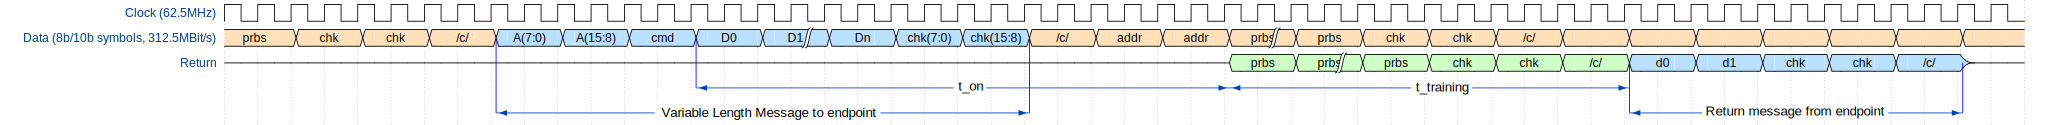
\includegraphics[width=\linewidth]{dts_sp-variable-length-message_ed.pdf}
	\caption{Example timing data stream for a variable length message. The preceding idle packet (also a variable length message) terminates in a /C/ (K28.5) character. The endpoint returns data to the timing master after a period $t_{\mathrm on}$ needed by the endpoint to activate its transmitter plus $t_{\mathrm training}$ needed by the timing master to lock to the signal.}
	\label{fig:wave-variable-length}
\end{figure}

\begin{figure}[h]
	\centering
	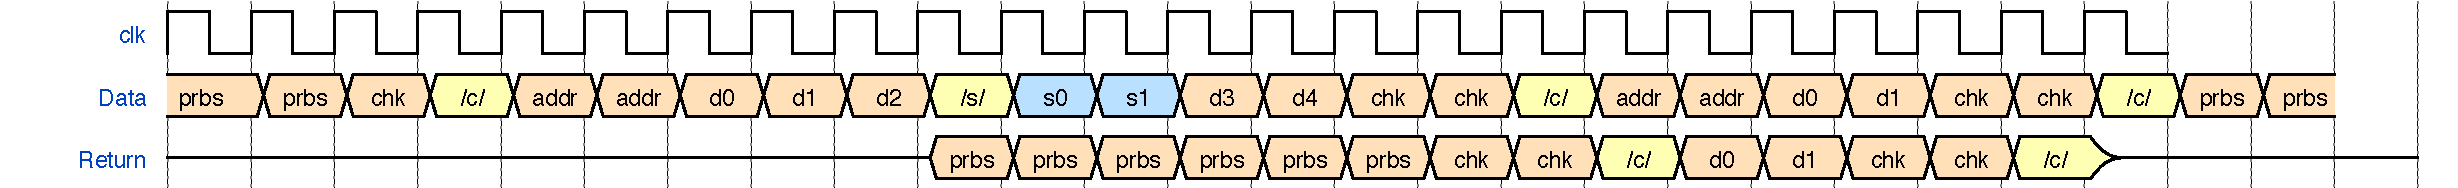
\includegraphics[width=\linewidth]{timing_protocol_wavedrom_01.pdf}
	\caption{Example timing data stream for a variable length message interrupted by a fixed length message. (Fixed length messages have higher priority than variable length).}
	\label{fig:wave-interupted-message}
\end{figure}
\end{landscape}


\subsection{Layer 2: Addressing and Protocol}

The synchronous and asynchronous packet formats are shown in Tables~\ref{tab:async} and \ref{tab:sync}.

\begin{table}[h!]
  \centering
  \begin{tabular}{@{}ll@{}} \toprule
    Byte & Content \\ \midrule
    0 & /S/ (K28.1) \\
    1 & Group / Command \\ \bottomrule
  \end{tabular}
  \caption{Fixed length packet format}
  \label{tab:sync}
\end{table}

\begin{table}[h!]
  \centering
  \begin{tabular}{@{}ll@{}} \toprule
    Byte & Content \\ \midrule
    0 & Address(7:0) \\
    1 & Address(15:8) \\
    2 & Command \\
    3 & Data byte 0 \\ 
    $3 + n$ & Data byte $n$ \\ 
    $3 + n + 1$ & Checksum(7:0) \\
    $3 + n + 2$ & Checksum(15:8) \\
    $3 + n + 3$ & /C/ (K28.5) \\ \bottomrule
  \end{tabular}
  \caption{Variable length packet format}
  \label{tab:async}
\end{table}

Fixed length packets contain a single four-bit timing group specifier, and a single four-bit command. The command field encodes sixteen separate synchronous commands, corresponding directly to the sync outputs of the decoder block. Every timing endpoint may be configured with a timing group mask, such that it accept fixed length (synchronous) commands addressed only to selected timing groups. This allows flexible partitioning of the system.

The timing protocol allows transmission of fixed length commands at a rate of no more than once per 10 clock cycles, which is adequate for the low rate of synchronous commands expected in both ProtoDUNE-SP and DUNE. In the event of clashing fixed length commands, a priority encoding scheme is used, such that lower-numbered commands preempt high-numbered ones, and lower-numbered timing groups preempt higher numbered ones. Under rare or pathological conditions this may result in a fixed length command being rejected; a record is kept of all propagated and rejected signals.

Variable length packets contain a single one-byte command followed by an arbitrary number of data bytes. The address is a unique experiment-wide 16b endpoint identifier, or has the special value of 0xfff in the top 12 bits for a broadcast packet, with the timing group identifier in the bottom four bits. The checksum is a standard CRC-16-CCITT, calculated on all packet bytes including the address. Return data packets lack the address field, but are otherwise identical. Idle packets are identified by the all-zeroes address, and contain random data which is not interpreted further by the endpoint, except to validate the checksum.

{\color{red}FUTURE\_UPDATE} Document the ProtoDUNE-SP address assignment. Document the ProtoDUNE-SP Run 2 address assignment. Document the DUNE address assignment.

\subsection{Layer 3: Command assignment}

Currently defined fixed length (synchronous) and variable length (asynchronous) commands are shown in Tables~\ref{tab:sync_cmds}, \ref{tab:async_cmds} and \ref{tab:async_ret_cmds}. In the case of fixed-length command queue conflict, priority for transmission is assigned to lower-numbered commands (i.e. counter sync command has priority over all over traffic). Variable length commands meant to be interpreted internally by the timing system endpoint decoder use are distinguished by a 0 in the topmost bit of the command byte.

\begin{table}[h!]
  \centering
  \begin{tabular}{@{}llp{9cm}@{}} \toprule
    Cmd bit & Name & Notes\\ \midrule
    0 & S\_Sync & Used to align and check system cycle counter; issued at 1ms intervals \\
    14 & S\_Spill & SPS spill warning toggle \\
    15 & S\_Trig & Beam trigger signal \\ \bottomrule
  \end{tabular}
  \caption{Fixed length commands}
  \label{tab:sync_cmds}
\end{table}

\begin{table}[h!]
  \centering
  \begin{tabular}{@{}lllp{9cm}@{}} \toprule
    Cmd & Name & Data bytes & Notes\\ \midrule
    0x0 & A\_Reset & 0 & Resets state of endpoint \\
    0x1 & A\_Sync & 8 & Stores cycle counter value to be loaded at next S\_Sync \\
    0x2 & A\_Enable & 0 & Enables endpoint transmission \\
    0x3 & A\_Status & 1 & Request endpoint status packet transmission \\ 
    0x4 & A\_Adjust & 2 & Adjusts packet delay and clock phase of endpoint \\ \bottomrule
  \end{tabular}
  \caption{Variable Length commands}
  \label{tab:async_cmds}
\end{table}

\begin{table}[h!]
  \centering
  \begin{tabular}{@{}lllp{9cm}@{}} \toprule
    Cmd & Name & Data bytes & Notes\\ \midrule
    0x0 & R\_Status & TBD & Endpoint status report \\ \bottomrule
  \end{tabular}
  \caption{Variable length return commands}
  \label{tab:async_ret_cmds}
\end{table}

{\color{red}FUTURE\_UPDATE} Define further synchronous and asynchronous commands.

\section{Timing Endpoint Interfaces}

\subsection{Timing Endpoint Functions}

A timing endpoint is characterised by the following properties:

\begin{itemize}
	\item A single system clock phase, adjustable under timing system control
	\item A unique address
	\item A timing group mask
\end{itemize}

A conceptual diagram of an endpoint is shown in Figure~\ref{fig:fw_if}. It consists of three major components and one optional component:

\begin{itemize}
	\item A clock and data recovery IC (e.g. ADN2814). This component is not required for endpoints with a clock + data interface.
	\item A PLL for jitter reduction and phase adjustment, with the latter function controlled from the endpoint FPGA. The PLL may be implemented as an internal clock controller (e.g. MMCM) within the FPGA, or may be an external component. This component is not required for endpoints with a clock + data interface, since phase may be controlled by the optical-LVDS converter module if necessary.
	\item A firmware protocol decoder, implemented inside the FPGA as part of the overall system firmware. This block receives and interprets the timing data stream, and provides decoded commands to other blocks inside the FPGA. It also monitors and counts errors observed in the data stream.
	\item(optional) For high precision phase alignment ( $< 1{\mathrm ns}$) a high speed D-type flip-flop should be used to re-time the outgoing data stream onto the master 312.5MHz clock.
\end{itemize}

Error conditions monitored by the decoder include:

\begin{itemize}
	\item 8b/10b decoder errors
	\item Packet checksum errors
	\item Counter-out-of-sync error
	\item CDR / PLL lock timeout
\end{itemize}

The status of the decoder may be monitored locally via the status flags (see below), or for soft errors, remotely via the R\_Status command. An endpoint that is in error can be reset locally or via the timing system, and then brought back into synchronisation with the rest of the system at the next S\_Sync command.

\begin{figure}[p]
	\centering
	\includegraphics[width=0.9\textwidth]{timing_endpoint_block.pdf}
	\caption{Endpoint signal paths}
	\label{fig:fw_if}
\end{figure}

\subsection{Endpoint Firmware Interface}

The decoder block exposes three sets of signals:

\subsubsection{\textcolor{red}{sys\_clk} domain signals}

\begin{itemize}
	\item |sys_clk| (o) is the free-running local clock provided by the host FPGA
	\item |sys_rst| (i) is a startup synchronous reset signal
	\item |address| (i) is a 32b word specifying: the address identifying this endpoint (see above for addressing scheme); and the timing group mask. It should not change once |sys_rst| is released.
	\item |status| (o, 4b) is a set of output signals indicating the internal state of the decoder, including: whether the core is in contact with the timing master; is in one of several possible setup or error conditions; is providing a stable global clock. The signal may be used to drive a reset of all logic governed by the global clock.
\end{itemize}

{\color{red}FUTURE\_UPDATE} Write state transition diagram for the decoder.

\subsubsection{\textcolor{red}{Global\_clk} domain signals}

\begin{itemize}
	\item |global_clk| (i) is the phase-adjusted 50MHz system clock from the PLL
	\item |sync| (o, 16b) is a set of bits corresponding to decoded fixed length messages. These bits go high for one clock cycle on receipt of the corresponding fixed length message.
	\item |cmd| (o, 8b) is a byte-wide output carrying a copy of received packet data addressed to this endpoint.
	\item |strobe| (o) is a signal qualifying the validity of the |cmd| output. It stays high for an entire packet of data, then goes low at the end of the packet.
	\item |timestamp| (o, 64b) is the 64b system cycle counter, cycling at global clock frequency.
\end{itemize}

\subsubsection{Other signals}

\begin{itemize}
	\item |data| (i) is the recovered or received serial timing data stream. This signal is automatically registered on the rising or falling edge of |global_clk| in order to cope with arbitrary phase alignment.
	\item |cdr_lock| (i) is the lock status signal of the CDR chip
	\item |pll_lock| (i) is the lock status of the PLL
	\item |pll_adj| (o, 8b) is a word indicating the desired phase adjustment for global\_clock. The physical interface to the PLL is implemented by the host FPGA, since this may require communication via a range of means to the PLL depending on implementation.
\end{itemize}

\section{System Level Operations}

The steps required to accomplish basic system level operations are listed below in simplified form. These steps are driven by software.

{\color{red}FUTURE\_UPDATE} Add calibration sequences as required.

\subsection{System Startup}

This procedure is carried out at system startup.

\begin{enumerate}
	\item Reset and initialise timing master unit
	\item Perform master self-test via timing path loopback
	\item Enable command transmission
\end{enumerate}

\subsection{Phase Adjustment}

This procedure is carried out after endpoints are powered and reset, but before final endpoint initialisation. It is assumed that a 'running' status from the timing decoder will be a necessary step in individual endpoint initialisation sequences. For each endpoint in turn, phase adjustment is carried out as follows:

\begin{enumerate}
	\item Enable endpoint transmission
	\item Wait for CDR lock and measure clock phase
	\item Request status packet
	\item Measure whole-cycle offset to establish path delay to / from endpoint
	\item Issue delay / phase adjustment command
	\item Verify correct alignment
	\item Disable endpoint transmission
\end{enumerate}

This process is estimated to require around 10ms per endpoint (dominated by the time required for CDR lock and clock phase measurement), allowing ProtoDUNE-SP to be brought up in a few seconds.

{\color{red}FUTURE\_UPDATE} Document measured phase adjustment time as measured in hardware.

\subsection{Operations Startup}

This procedure is carried out after all endpoints are aligned, and after time-of-day is established via GPS.

\begin{enumerate}
	\item Reset master cycle counter
	\item Enable command and input logging
	\item Enable regular S\_Sync commands
	\item Enable trigger commands
\end{enumerate}

\subsection{System Monitoring}

System monitoring is continually carried out by continuous repetition of the endpoint phase check sequence, and logging of any error counts reported by endpoints. This activity has lower priority than other system activities.

\subsection{Operations Shutdown}

This procedure is carried out after all DAQ queues have drained, as one of the last end-of-run steps.

\begin{enumerate} 
	\item Disable trigger commands
	\item Wait until next S\_Sync command
	\item Disable regular S\_Sync commands
	\item Issue S\_Reset
	\item Disable command and input logging
\end{enumerate}

\clearpage

\appendix

\section{DTS-SP Firmware, Software}

At the time of writing, DTS-SP firmware is hosted at \url{https://gitlab.cern.ch/protoDUNE-SP-DAQ/timing-board-firmware} . Scripts to test and configure the timing system firmware are hosted at \url{https://gitlab.cern.ch/protoDUNE-SP-DAQ/timing-board-software}



\section{Example Endpoint Firmware}

\subsection{Interface to Example Endpoint Firmware }

The top-level declaration for the endpoint entity is:

\begin{minted}{vhdl}
entity pdts_endpoint is
  generic(
    SCLK_FREQ : real    := 62.5;        -- Frequency (MHz) of the supplied sclk
                                        -- ( 62.5MHz for DUNE , 50MHz for ProtoDUNE-1 )
    EN_TX     : boolean := false        -- Enable endpoint to originate messages.
                                        -- Only for ETI (CTB in ProtoDUNE-1)
    );
  port(
    sclk       : in  std_logic;         -- Free-running system clock
    srst       : in  std_logic;         -- System reset (sclk domain)
    addr       : in  std_logic_vector(7 downto 0);  -- Endpoint address
                                                    -- (async, sampled in clk domain)
    tgrp       : in  std_logic_vector(1 downto 0);  -- Timing group
                                                    -- (async, sampled in clk domain)
    stat       : out std_logic_vector(3 downto 0);  -- Status output (sclk domain)
    rec_clk    : in  std_logic;         -- CDR recovered clock from timing link
    rec_d      : in  std_logic;         -- CDR recovered data from timing link
                                        -- (rec_clk domain)
    txd        : out std_logic;         -- Output data to timing link
                                        -- (rec_clk domain)
    sfp_los    : in  std_logic := '0';  -- SFP LOS line
                                        -- (async, sampled in sclk domain)
    cdr_los    : in  std_logic := '0';  -- CDR LOS line
                                        -- (async, sampled in sclk domain)
    cdr_lol    : in  std_logic := '0';  -- CDR LOL line
                                        -- (async, sampled in sclk domain)
    sfp_tx_dis : out std_logic;         -- SFP tx disable line (clk domain)
    clk        : out std_logic;         -- 62.5MHz clock output
    rst        : out std_logic;         -- 62.5MHz domain reset
    rdy        : out std_logic;         -- Timestamp valid flag
    sync       : out std_logic_vector(SCMD_W - 1 downto 0);  -- fixed-length command
                                                             -- output (clk domain)
    sync_stb   : out std_logic;         -- fixed length command strobe (clk domain)
    sync_valid : out std_logic;         -- fixed length command valid flag (clk domain)
    tstamp     : out std_logic_vector(8 * TSTAMP_WDS - 1 downto 0);  -- Timestamp out
    tsync_in   : in  cmd_w     := CMD_W_NULL;       -- Tx fixed-length command input
    tsync_out  : out cmd_r              -- Tx fixed-length command handshake
    );


end pdts_endpoint;
\end{minted}

Where the ports are as described below:

\begin{itemize}
    

\item |SCLK_FREQ| should be set to the frequency of the supplied system clock ``sclk'' in MHz

\item |EN_TX| should be left at the default of false unless the endpoint is to be a source of messages rather than responding to them. Only set true for ETI in DUNE, or CTB in ProtoDUNE

\item |sclk| is a free-running system clock at a frequency of your choice. There is no clock
buffering or other manipulation inside the endpoint block.

\item |srst| is a synchronous reset (|sclk| domain) that should be held high until |sclk |is stable
and the configuration signals to the endpoint are ready. Asserting this signal will cause
the endpoint to begin its initialisation sequence again

\item |addr| is an eight-bit address that should be unique for each endpoint in the system.
Set to all-zeroes for now.

\item |tgrp| is a two-bit address that sets the timing group (or 'partition') that this instance
of the endpoint is a member of. You probably need to set this from a register in your
design.

\item |stat| (|sclk| domain) indicates the status of the endpoint (you can find the meaning of the states
in |pdts_ep_startup.vhd|. This is provided only for debugging purposes. You should use the
|rdy| signal to indicate to your firmware when the signals from the endpoint are valid.

\item |rec_clk| is the recovered clock from the CDR device (or from the clock line in case of separate clock and data lines)

\item |rec_d| is the recovered data from the CDR device (or from the serial data line in case of separate clock and data).

\item |txd| is the output data from the endpoint back to the master. Register this with the your local DTS-SP clock and connect to your
SFP data input (or the ``copper'' signal lines if using direct connection).

\item |sfp_los| should be connected to the corresponding line on the SFP (for systems
not using an SFP, leave unconnected).

\item |cdr_los| should be connected to the corresponding line on the CDR chip (for systems not using
CDR, leave unconnected).

\item |cdr_lol| should be connected to the corresponding line on the CDR chip (for systems not using
CDR, leave unconnected).

\item |sfp_tx_dis| should be connected to the corresponding transmit disable line on the SFP

\item |clk| is the phase-adjusted 62.5MHz DUNE (50MHz ProtoDUNE) system clock

\item |rst| is a synchronous reset (|clk| domain) to your logic, asserted until the phase of |clk|
is stable.

\item |rdy| (|clk| domain) indicates that the endpoint is running, and that output signals are
valid. Until |rdy| is asserted, the |tstamp| may change randomly, and sync commands are
meaningless.

\item |sync| (|clk| domain) is the fixed-length (synchronous) command output from the endpoint. The table of current
command codes can be found in |pdts_defs.vhd|.

\item |sync_stb| (|clk| domain) is the strobe for sync, and is asserted each time a new data word is
written to sync. Note that commands can be longer than one word long.

\item |sync_valid| (|clk| domain) is asserted on the first word of each fixed-length command. If your firmware only
cares about the first word of each command (e.g. if you only listen to trigger
commands, you can treat this as the qualifying signal for sync, and ignore
subsequent words of commands).

\item |tstamp| (|clk| domain) is the system-wide 64b timestamp.

\item |tsync_in| (|clk| domain) is the interface for sending fixed length (synchronous) commands back to the master, and should
only be used by the ETI in DUNE (CTB in ProtoDUNE). Others should leave it disconnected.

\item |tsync_out| (|clk| domain) is the handshaking signals accompanying |tsync_in|, and should
only be used by the ETI in DUNE (CTB in ProtoDUNE).

\end{itemize}

In order to assist in decoding the fixed length commands at ProtoDUNE-1, a utility block is provided in
|components/pdts/firmware/hdl/pdts_ep_decoder.vhd|:

\begin{minted}{vhdl}
entity pdts_ep_decoder is
  port(
    clk      : in  std_logic;           -- 62.5MHz clock (50MHz ProtoDUNE)
    rst      : in  std_logic;           -- Sync reset
    rdy      : in  std_logic;           -- Timing system up flag
    scmd     : in  std_logic_vector(SCMD_W - 1 downto 0);  -- fixed length
                                                           -- command input
    scmd_v   : in  std_logic;           -- fixed length command valid flag
    in_spill : out std_logic;           -- Spill flag (ProtoDUNE)
    in_run   : out std_logic;           -- Run flag (ProtoDUNE)
    evtctr   : out std_logic_vector(8 * EVTCTR_WDS - 1 downto 0)  -- Event counter
    );

\end{minted}
\clearpage
\printbibliography

\end{document}
 